\documentclass[11pt]{article}
\usepackage[margin=1in]{geometry}
\usepackage{amsmath,amssymb,amsthm}
\usepackage{graphicx}
\usepackage[hidelinks]{hyperref}

\newtheorem{proposition}{Proposition}
\newtheorem{corollary}{Corollary}
\theoremstyle{definition}
\newtheorem{definition}{Definition}
\newtheorem{remark}{Remark}

\newcommand{\opt}{\mathrm{opt}}
\newcommand{\best}{\mathrm{best}}

\title{The Value of an Agora: A Simple Start}
\author{Nimrod Talmon}
\date{Draft, November 2026}

\begin{document}
\maketitle

\begin{abstract}
Soon, many people will have a personal AI agent. Each agent can ask its person questions, but every question costs the person attention. We ask what agents gain by working together rather than alone. We study the simplest case: a community picks one option, and each agent may ask its person only a few yes/no questions. Agents that work alone can guarantee only a fraction of the best outcome, equal to the number of questions divided by the number of options, and no more. Agents that share their answers can reach the best outcome with two questions each in the hardest case for agents working alone; sharing costs messages, few through a coordinator and many without one.
\end{abstract}

\section{The Story}

A neighborhood wants to start one activity: a community garden, a carpool, a book club, or one of several others.
Each resident has a personal AI agent.
To know who would join which activity, an agent must ask its resident, and residents do not want to answer many questions.
So each agent may ask only a few.

If each agent works alone, then it asks its resident about a few activities and reports the answers.
Suppose that every resident would join the garden, and no one would join anything else.
An agent working alone does not know this, so it finds the garden only if it happens to ask about it; with two questions and ten activities, about one agent in five does.

If the agents share what they learn, then one agent that hears ``yes, the garden'' is enough: every other agent asks its resident about the garden, and everyone joins.
Two questions per resident suffice: one to search together, and one to join.

This note makes this story precise.
Agents that work alone can guarantee exactly the share of the best outcome given by the number of questions divided by the number of options (Proposition~\ref{prop:silos}).
Agents that share their answers reach the best outcome in the example above (Proposition~\ref{prop:central}), so this is the largest gain that sharing can bring (Corollary~\ref{cor:value}).
Sharing costs messages: few when the agents talk through a coordinator, and many when they talk to each other directly (Proposition~\ref{prop:grassroots}).

\section{The Model}

\begin{definition}[Community]
A community consists of $n$~members and $m$~options.
Each member~$i$ approves a set of options, unknown to everyone, including the member's agent.
\end{definition}

\begin{definition}[Agents and questions]
Each member~$i$ has an agent, agent~$i$.
Agent~$i$ may ask member~$i$ a question ``do you approve option~$o$?''; the member answers truthfully.
Each question costs member~$i$ one unit of attention, and each agent may ask its member at most $b$~questions; $b$ is the \emph{budget}.
\end{definition}

\begin{definition}[Outcome and welfare]
An outcome is an option~$o$ together with a set of \emph{enrolled} members, each of whom answered ``yes'' to the question about~$o$.
The \emph{welfare} of an outcome is the number of its enrolled members.
The optimum $\opt$ is the largest number of members that approve a single option.
\end{definition}

\begin{definition}[Settings]
\emph{Silos:} each agent asks its questions without any information about the other members, and then sends its member's answers to a mechanism, which outputs an outcome.
\emph{Central Agora:} a coordinator decides which member is asked which question, based on all answers so far, and outputs an outcome; each question and each answer is a message between the coordinator and an agent.
\emph{Grassroots Agora:} agents send messages directly to each other, each agent decides what to ask and what to send based only on its own member's answers and the messages it received, and all agents must output the same outcome.
Agents act in synchronous rounds.
\end{definition}

\begin{definition}[Guarantees and the value of the Agora]
A protocol \emph{guarantees} a ratio~$r$ on a class of instances if, on every instance in the class, its expected welfare is at least $r \cdot \opt$.
For a setting~$S$, $\best_S(b)$ is the largest ratio that a protocol in~$S$ with budget~$b$ guarantees.
The \emph{value of the central Agora} is $\best_{\text{central}}(b) / \best_{\text{silos}}(b)$, and the value of the grassroots Agora is defined in the same way.
\end{definition}

\begin{definition}[Hidden favorite]
In a \emph{hidden-favorite} instance, all members approve one option, the favorite, and no member approves any other option.
\end{definition}

\begin{remark}
Enrolling only members who said ``yes'' means that an agent commits its member to nothing that the member did not confirm.
Without this requirement, a mechanism that learned the favorite from one member could enroll everyone, and the questions would lose their meaning.
\end{remark}

\begin{remark}
The two costs of a protocol are kept apart: attention, the number of questions, which takes people's time, and messages, which take only computation.
Rounds cost nothing here.
\end{remark}

\section{Results}

\begin{proposition}[Silos]\label{prop:silos}
Let $1 \le b \le m$.
In silos, the protocol in which every agent asks about $b$~options chosen uniformly at random, and the mechanism picks the option with the most ``yes'' answers, guarantees the ratio~$b/m$ on all instances.
No protocol in silos guarantees more than $b/m$, already on hidden-favorite instances.
Hence $\best_{\text{silos}}(b) = b/m$.
\end{proposition}

\begin{proof}
For the first part, fix an instance and an option~$o^\ast$ that $\opt$~members approve.
Each of them asks about~$o^\ast$ with probability~$b/m$, so the expected number of ``yes'' answers about~$o^\ast$ is $(b/m)\cdot\opt$.
The mechanism picks an option with at least as many ``yes'' answers as~$o^\ast$ and enrolls exactly the members who said ``yes'' to it, so its expected welfare is at least $(b/m)\cdot\opt$.

For the second part, fix a protocol in silos and run it on the hidden-favorite instance with favorite~$f$.
Until agent~$i$ asks about~$f$, every answer it gets is ``no'', whatever~$f$ is.
So the options that agent~$i$ asks about before it asks about~$f$ follow one random sequence, the sequence the agent would follow if all answers were ``no'', and this sequence does not depend on~$f$.
Agent~$i$ asks about~$f$ only if $f$~is among the first $b$~options of this sequence.
If $f$~is chosen uniformly at random, then this happens with probability at most~$b/m$.
Only members who said ``yes'' to the chosen option can be enrolled, and on this instance only members who were asked about~$f$ said ``yes'' to anything, so the expected welfare is at most $n \cdot b/m$ for a random favorite.
Hence for some favorite~$f$ the expected welfare is at most $n \cdot b/m = (b/m)\cdot\opt$.
\end{proof}

\begin{proposition}[Central Agora]\label{prop:central}
Let $n \ge m$ and $2 \le b \le m$.
In the central Agora, the following protocol enrolls all $n$~members on every hidden-favorite instance.
\emph{Explore:} member~$i$ is asked about the $b-1$ options $i, i+1, \dots, i+b-2$, counted modulo~$m$.
\emph{Commit:} the leader is the option with the largest share of ``yes'' answers among the members asked about it; every member not yet asked about the leader is asked about it; the outcome is the leader, with the members who said ``yes'' to it.
The protocol asks at most $n \cdot b$ questions and sends two messages per question.
\end{proposition}

\begin{proof}
Since $n \ge m$, every option is asked about during exploration, including the favorite~$f$.
The members asked about~$f$ say ``yes'', and every other answer is ``no'', so $f$~is the only option with a positive share of ``yes'' answers, and it becomes the leader.
Each member not yet asked about~$f$ has asked $b-1$ questions, so it has one question left, and it is asked about~$f$.
All members approve~$f$, so all of them say ``yes'' and all are enrolled.
\end{proof}

\begin{corollary}\label{cor:value}
Let $n \ge m$ and $2 \le b \le m$.
On hidden-favorite instances, the value of the central Agora is $m/b$.
On all instances, the value of the central Agora is at most $m/b$.
\end{corollary}

\begin{proof}
On hidden-favorite instances, Proposition~\ref{prop:central} gives $\best_{\text{central}}(b) = 1$ and Proposition~\ref{prop:silos} gives $\best_{\text{silos}}(b) = b/m$.
On all instances, $\best_{\text{central}}(b) \le 1$ and, by Proposition~\ref{prop:silos}, $\best_{\text{silos}}(b) = b/m$.
\end{proof}

\begin{proposition}[Grassroots Agora]\label{prop:grassroots}
Under the conditions of Proposition~\ref{prop:central}, the same outcome is reached without a coordinator.
Each agent asks the exploration questions of Proposition~\ref{prop:central}, which depend only on its own index, and sends every ``yes'' answer of its member to all other agents.
After exploration, every agent computes the same leader from the ``yes'' answers it received, asks its member about the leader if it has not yet done so, and again sends a ``yes'' answer to all other agents.
All agents output the leader with the members who said ``yes'' to it.
On hidden-favorite instances, this protocol enrolls all members and sends $n(n-1)$ messages, whereas the protocol of Proposition~\ref{prop:central} sends at most $4n$ messages when $b = 2$.
\end{proposition}

\begin{proof}
The exploration plan is known to all agents, so an agent that receives no ``yes'' from member~$j$ about option~$o$ knows that member~$j$ was not asked about~$o$ or said ``no''.
Hence all agents see the same ``yes'' answers, compute the same leader, and output the same outcome; by the argument of Proposition~\ref{prop:central}, the leader is the favorite and all members are enrolled.
Each member says ``yes'' exactly once, to the favorite, and each ``yes'' is sent to $n-1$~agents, so $n(n-1)$ messages are sent.
With $b = 2$, the central protocol asks at most $2n$ questions and sends two messages per question.
\end{proof}

\begin{remark}
With a budget of one question, the central Agora can still do well, because rounds cost nothing: it asks members one at a time about distinct options until one says ``yes'', and then asks all remaining members about that option.
On hidden-favorite instances, this enrolls at least $n-m+1$ members, whereas silos guarantee only $1/m$ of the optimum.
\end{remark}

\section{Simulation}

Figure~\ref{fig:sim} shows the protocols of Propositions~\ref{prop:silos}--\ref{prop:grassroots} on communities of $40$~members and $10$~options, averaged over $50$~instances per point.
On hidden-favorite instances, silos follow the line $b/m$ and the Agora reaches the optimum from two questions on.
On instances in which each option~$o$ is approved by each member independently with a probability drawn uniformly between $0$ and~$0.6$, silos do slightly better than $b/m$, and the Agora reaches $81\%$ of the optimum with two questions per member (silos: $26\%$) and $93\%$ with five (silos: $54\%$).
The central and grassroots Agoras reach the same outcomes; with two questions per member, the central Agora sends $152$~messages on average and the grassroots Agora $1087$.

\begin{figure}[t]
\centering
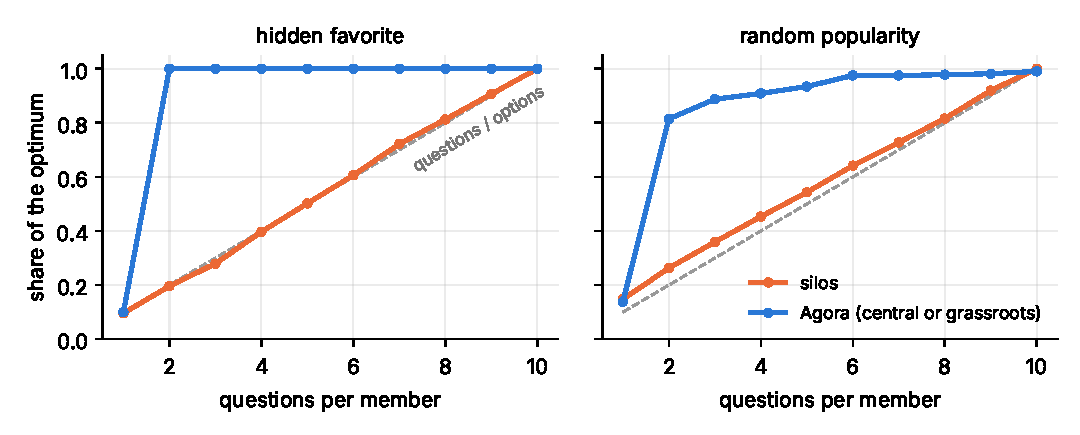
\includegraphics[width=\linewidth]{pick_one.pdf}
\caption{Share of the optimum reached, by questions per member; $40$~members, $10$~options, $50$~instances per point. The dashed line is the number of questions divided by the number of options.}
\label{fig:sim}
\end{figure}

\section{Outlook}

\begin{remark}
On all instances, the central Agora's guarantee is open.
Explore-then-commit is close to the optimum on random instances, but a worst-case guarantee needs care: an option that a small sample makes look good may be worse than one that it makes look bad.
Choosing which options to ask about, based on the answers so far, resembles choosing which arm to pull in a bandit problem, with a twist: here the ``yes'' answers about the chosen option are themselves the welfare.
\end{remark}

\begin{remark}
Natural next steps, each a small change to the model: an option runs only if enough members join; several options run at once and each member joins at most one, which is forming groups; agents start knowing part of what their members approve, so that they can answer some questions themselves; grassroots protocols that send fewer messages; and agents that act strategically for their members.
\end{remark}

\end{document}
